\subsection{الخوارزمية المقترحة لروبوت واحد}

تعتمد الخوارزمية المقترحة لإنتاج طريق يسلكه الروبوت في بيئته على انشاء حقل سرعة يمكن للروبوت الانحدار فيه مشكلاً طريقه الخاص. نعتمد هنا على انشاء هذا الحقل عن طريق حل المعادلة التفاضلية الجزئية لتدفق السوائل الغير قابلة للانضغاط من نقطة الى أخرى.
أولاً، نكتب معادلات نافيير-ستوكس بشكلها المتجهي الخاصة بالموائع غير القابلة للانضغاط:




\begin{equation}
 \nabla \cdot \vec{\upsilon} = 0  
\end{equation}

\begin{equation}
 \frac{\partial \upsilon }{\partial t} +  \left(\vec{\upsilon }\cdot\nabla\right)\vec{\upsilon } = -\frac{1}{\rho}\nabla p+\nu\nabla^2\vec{\upsilon } 
\end{equation}

حيث $\vec{\upsilon } = (u,v,w)^T$ مركبات السرعة على المحاور الإحداثية الثلاث.

المعادلة الأولى تمثل انحفاظ الكتلة عند ثبات الكثافة (عدم الانضغاطية)، وتمثل المعادلة الثانية انحفاظ العزم. في الموائع غير الانضغاطية، معادلة انحفاظ الكتلة تخلق قيد كينيماتيكي يتطلب من حقل الضغط أن يتغير بشكل يسمح ل معدل تغير السرعة $\nabla \cdot \vec{\upsilon}$ بالانعدام في كل نقاط الفضاء. يمكن بناء حقل الضغط بأخذ تباعد (divergence) معادلة العزم، بعد أخد هذه الخطوة تظهر معادلة بواسون للضغط.


نعيد كتابة معادلات نافيير-ستوكس بشكل مريح للتقطيع وذلك بعد تعويض $ w=0 $:

\begin{equation}\label{eq:11:3}
\frac{\partial u}{\partial t}+u\frac{\partial u}{\partial x}+v\frac{\partial u}{\partial y}=-\frac{1}{\rho}\frac{\partial p}{\partial x}+\nu\left(\frac{\partial^2u}{\partial x^2}+\frac{\partial^2u}{\partial y^2}\right)
\end{equation}

\begin{equation}\label{eq:11:4}
\frac{\partial v}{\partial t}+u\frac{\partial v}{\partial x}+v\frac{\partial v}{\partial y}=-\frac{1}{\rho}\frac{\partial p}{\partial y}+\nu\left(\frac{\partial^2v}{\partial x^2}+\frac{\partial^2v}{\partial y^2}\right)
\end{equation}

\begin{equation}\label{eq:11:5}
\frac{\partial^2p}{\partial x^2}+\frac{\partial^2p}{\partial y^2}=-\rho\left(\frac{\partial u}{\partial x}\frac{\partial u}{\partial x}+2\frac{\partial u}{\partial y}\frac{\partial v}{\partial x}+\frac{\partial v}{\partial y}\frac{\partial v}{\partial y}\right)
\end{equation}


نتجه الآن لإنشاء mesh خاص بالمكان يسمح لنا بحل هذه المعادلات بيسر. اتجهنا لاستخدام تقطيع المكان الى مربعات لسهولة برمجتها. تظهر الصورة في الملحق رقم 1 تقطيع لحلبة مولدة عشوائياً. بعد تقطيع الحلبة يمكن بسهولة نقل \ref{eq:11:3} , \ref{eq:11:4} , \ref{eq:11:5} الى المتقطع بالشكل:

\begin{equation}
\begin{matrix}&\frac{u_{i,j}^{n+1}-u_{i,j}^n}{\Delta t}+u_{i,j}^n\frac{u_{i,j}^n-u_{i-1,j}^n}{\Delta x}+v_{i,j}^n\frac{u_{i,j}^n-u_{i,j-1}^n}{\Delta y}=\\&-\frac{1}{\rho}\frac{p_{i+1,j}^n-p_{i-1,j}^n}{2\Delta x}+\nu\left(\frac{u_{i+1,j}^n-2u_{i,j}^n+u_{i-1,j}^n}{\Delta x^2}+\frac{u_{i,j+1}^n-2u_{i,j}^n+u_{i,j-1}^n}{\Delta y^2}\right)\\\end{matrix}
\end{equation}

\begin{equation}
\begin{matrix}&\frac{v_{i,j}^{n+1}-v_{i,j}^n}{\Delta t}+u_{i,j}^n\frac{v_{i,j}^n-v_{i-1,j}^n}{\Delta x}+v_{i,j}^n\frac{v_{i,j}^n-v_{i,j-1}^n}{\Delta y}=\\&-\frac{1}{\rho}\frac{p_{i,j+1}^n-p_{i,j-1}^n}{2\Delta y}+\nu\left(\frac{v_{i+1,j}^n-2v_{i,j}^n+v_{i-1,j}^n}{\Delta x^2}+\frac{v_{i,j+1}^n-2v_{i,j}^n+v_{i,j-1}^n}{\Delta y^2}\right)\\\end{matrix}
\end{equation}




\begin{equation}
\begin{matrix}

\frac{p_{i+1,j}^n-2p_{i,j}^n+p_{i-1,j}^n}{\Delta x^2}+\frac{p_{i,j+1}^n-2p_{i,j}^n+p_{i,j-1}^n}{\Delta y^2} =


\\

\frac{\rho}{\Delta t}\left(\frac{u_{i+1,j}-u_{i-1,j}}{2\Delta x}+\frac{v_{i,j+1}-v_{i,j-1}}{2\Delta y}\right)-\frac{u_{i+1,j}-u_{i-1,j}}{2\Delta x}\frac{u_{i+1,j}-u_{i-1,j}}{2\Delta x} - 
\\
2\rho \frac{u_{i,j+1}-u_{i,j-1}}{2\Delta y}\frac{v_{i+1,j}-v_{i-1,j}}{2\Delta x}-\frac{v_{i,j+1}-v_{i,j-1}}{2\Delta y}\frac{v_{i,j+1}-v_{i,j-1}}{2\Delta y}

\end{matrix}
\end{equation}

بإعادة ترتيب المعادلات السابقة يمكن الحصول على الأطراف المتقدمة زمنياً:

\begin{equation}
\begin{matrix}u_{i,j}^{n+1}=u_{i,j}^n-u_{i,j}^n\frac{\Delta t}{\Delta x}(u_{i,j}^n-u_{i-1,j}^n)-v_{i,j}^n\frac{\Delta t}{\Delta y}(u_{i,j}^n-u_{i,j-1}^n)\\-\frac{\Delta t}{\rho2\Delta x}(p_{i+1,j}^n-p_{i-1,j}^n)\\+\nu\left(\frac{\Delta t}{\Delta x^2}\left(u_{i+1,j}^n-2u_{i,j}^n+u_{i-1,j}^n\right)+\frac{\Delta t}{\Delta y^2}\left(u_{i,j+1}^n-2u_{i,j}^n+u_{i,j-1}^n\right)\ \right)\\\end{matrix}
\end{equation}

\begin{equation}
\begin{matrix}v_{i,j}^{n+1}=v_{i,j}^n-u_{i,j}^n\frac{\Delta t}{\Delta x}\left(v_{i,j}^n-v_{i-1,j}^n\right)-v_{i,j}^n\frac{\Delta t}{\Delta y}\left(v_{i,j}^n-v_{i,j-1}^n\right)\ \ \\-\frac{\Delta t}{\rho2\Delta y}\left(p_{i,j+1}^n-p_{i,j-1}^n\right)\\+\nu\left(\frac{\Delta t}{\Delta x^2}\left(v_{i+1,j}^n-2v_{i,j}^n+v_{i-1,j}^n\right)+\frac{\Delta t}{\Delta y^2}\left(v_{i,j+1}^n-2v_{i,j}^n+v_{i,j-1}^n\right)\ \right)\\\end{matrix}
\end{equation}

\begin{equation}
\begin{matrix}
p_{i,j}^{n+1}=\frac{\left(p_{i+1,j}^n+p_{i-1,j}^n\right)\Delta y^2+\left(p_{i,j+1}^n+p_{i,j-1}^n\right)\Delta x^2}{2\left(\Delta x^2+\Delta y^2\right)}\ -\frac{\rho\Delta x^2\Delta y^2}{2\left(\Delta x^2+\Delta y^2\right)}
\\
\times\biggl[\frac{1}{\Delta t}\left(\frac{u_{i+1,j}-u_{i-1,j}}{2\Delta x}+\frac{v_{i,j+1}-v_{i,j-1}}{2\Delta y}\right)-\frac{u_{i+1,j}-u_{i-1,j}}{2\Delta x}\frac{u_{i+1,j}-u_{i-1,j}}{2\Delta x}\\-2\frac{u_{i,j+1}-u_{i,j-1}}{2\Delta y}\frac{v_{i+1,j}-v_{i-1,j}}{2\Delta x}-\frac{v_{i,j+1}-v_{i,j-1}}{2\Delta y}\frac{v_{i,j+1}-v_{i,j-1}}{2\Delta y}\biggr]

\end{matrix}
\end{equation}


\subsubsection{شروط المسألة: }
\begin{itemize}
	\item السرعة الابتدائية والضغط الابتدائي معدومان.
	\item السرعة معدومة عند الجدران .
	\item مشتق الضغط المكاني معدوم عند الجدران.
	\item الضغط +a عند نقطة انطلاق الروبوت -a عند الهدف.
	\item الضغط صفر عند الجدران.
\end{itemize}

بالحل الرقمي الـiterative يمكن الحصول على الحالة الثابتة steady state للمائع بعد عدد معين من التكرارات حيث يتم حساب السرعات المتقدمة بزمن قدره $\Delta t$. يمكن اختبار الوصول الى الحالة الثابتة من عدمه عن طريق معاينة $ \frac{dv}{dt}\ ,\frac{du}{dt} $ في كل iteration وانهاء الحساب عند هبوطه عن حد معين $ \epsilon $. عند الحصول على الحل النهائي نقوم بجعل الروبوت ينحدر باستخدام الحقل المتجهي الناتج موصلاً نفسه الى الهدف بشكل مباشر.
عند انشاء حقل السرعة لخريطة بأبعاد $ 100\times100  $ يستغرق الحاسوب الموصوف في ما متوسطه 500 ميلي ثانية. نذكر هنا أن هذا الزمن لا يعبر عن أصغر زمن يمكن للنظام انتاج حقل به، فهو لم يتعرض لأمثلة من هذه النواحي بعد:
\begin{itemize}
	\item شكل التقطيع.
	\item المعاملات الفيزيائية للمائع.
	\item التسريع باستخدام العتاد الصلب \textenglish{(Hardware Acceleration)}.
	
\end{itemize}


نوضح فيما يلي أمثلة عن حل الخوارزمية لعدة فضاءات عمل:

\begin{center}
	\centering
\begin{table}[ht]
	\begin{tabular}{cc}
		\begin{subfigure}{0.4\textwidth}\centering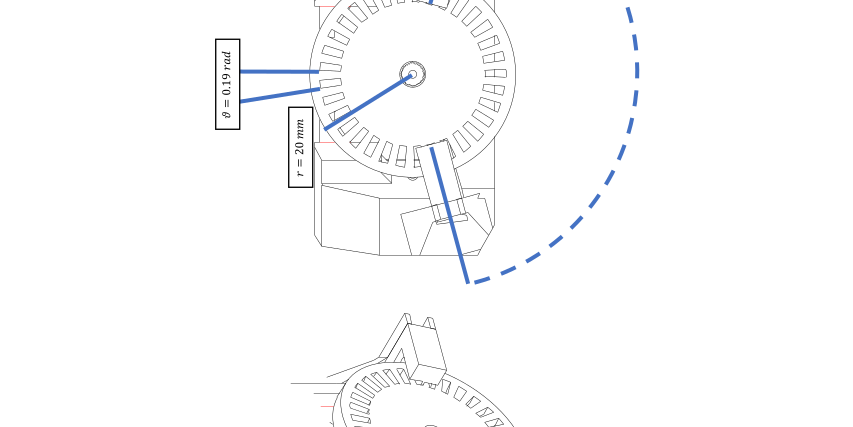
\includegraphics[width=0.9\linewidth]{figs/11/fig1}\caption{الخريطة الأولى}\label{11:fig:1}\end{subfigure}&
		\begin{subfigure}{0.4\textwidth}\centering\includegraphics[width=0.9\linewidth]{figs/11/fig2}\caption{الخريطة الثانية}\label{11:fig:2}\end{subfigure}\\
		\newline
		\begin{subfigure}{0.4\textwidth}\centering\includegraphics[width=0.9\linewidth]{figs/11/fig3}\caption{الخريطة الثالثة}\label{11:fig:3}\end{subfigure}&
		\begin{subfigure}{0.4\textwidth}\centering\includegraphics[width=0.9\linewidth]{figs/11/fig4}\caption{الخريطة الرابعة}\label{11:fig:4}\end{subfigure}\\
	\end{tabular}
	\caption{أداء الخوارزمية لعدة خرائط}
	\label{tab:mytable}
\end{table}
\end{center}


\subsection{الخوارزمية المقترحة للسرب}

أفضت الطريقة المتبعة في انتاج مسار لروبوت واحد في فضاء اختياري نتائج عالية الوثوقية والأمان، التجارب أثبتت بشكل كبير قدرة هذه الطريقة على إنتاج طريق ناعم حال وجود اتصال بين المبدأ والهدف. يعد تعميم هذه الطريقة لضمان وصول مجموعة روبوتات إلى هدفها عملية غاية في التعقيد، وذلك خصوصاً لطبيعة الروبوتات الغير هولنومية المدروسة في هذا المشروع. يمكن الاستدلال إلى تهجين بين عدة طرق لإيجاد ما يناسب حالات خاصة من فضاءات اعمل في الدراسات المرجعية.
لنتمكن من انتاج حل يتسم بالبساطة الاستدلالية وبالحتمية والكمالية، يجب العودة إلى الآلية التي تتصرف فيها جزيئات سائل وجدت نفسها في حقل كموني. إن ألية التفكير هذه تفضي إلى نوعين من الحلول:

\begin{itemize}
	\item الروبوتات غير واعية لبعضها
	\item الروبوتات (الجزيئات) واعية لبعضها
\end{itemize}

يمكن مقاربة الحل الأول بجزيئات سائل لا نيوتوني تسير في حقل السرعة المنتج، والطريقة الثانية بعدد من الأجسام صلبة تهوي في هذا الحقل.

\subsubsection{الروبوتات غير الواعية لوجود السرب}

هنا يتم احتساب حقل كموني صغير خارج من كل روبوت في السرب وإضافة هذه الحقول إلى حقل السرعة منهاً للتصادم، يتم هنا احتساب جميع قيم السرعة في كل نقاط الفضاء عن طريق أخذ جريان المائع من جهة والجيران من جهة أخرة. يمكن التحكم بقوة الحقل الكموني النافر الصادر عن كل روبوت بتغيير بارامترات الحساب.
ألية الحساب:

يتم أولاً ملء الخريطة فارغة بأجسام تتناسب أبعادها مع أبعاد الروبوتات الباقية في السرب، ثم يتم حساب تحويل المسافة للمصفوفة الناتجة \textenglish{(distance transform).} يتبع هذه الخطوة القيام بعملية مشروحة في الجدول \ref{11:fig:process}.





	\begin{table}
		\centering
		\begin{tabular}{cp{150pt}}
			\begin{subfigure}{0.35\textwidth}
				\centering
				\includesvg[width=0.9\linewidth]{figs/11/fig5}
			\end{subfigure}&  انشاء مصفوفة بأبعاد الخريطة ياوضع عليها الروبوتات الباقية من السرب. أبعاد الروبوتات في المصفوفة يتناسب مع أبعاد الروبوت (المصفوفة $\mathcal{M}$) \\
			\begin{subfigure}{0.35\textwidth}
				\centering
				\includesvg[width=0.9\linewidth]{figs/11/fig6}
			\end{subfigure}& التحويل المسافي $D(\mathcal{M})$\\
			\begin{subfigure}{0.35\textwidth}
				\centering
				\includesvg[width=0.9\linewidth]{figs/11/fig7}
			\end{subfigure}&  $\mathcal{M}_2 = \epsilon (1/D(\mathcal{M}) - 1/k )^2$ \\
			\begin{subfigure}{0.35\textwidth}
				\centering
				\includesvg[width=0.9\linewidth]{figs/11/fig8}
			\end{subfigure}& $ \mathcal{M}_2 > k $ \\
			\begin{subfigure}{0.35\textwidth}
				\centering
				\includesvg[width=0.9\linewidth]{figs/11/fig9}
			\end{subfigure}& $ \nabla (\mathcal{M}_2 > k) $
		\end{tabular}
		\caption{عملية حساب المسار في الحالة الأولى من الحل}
		\label{11:fig:process}
	\end{table}


ثم يتم جمع الحقل الناتج إلى حقول السرعة وإنتاج الحقل الخاص بكل روبوت. انزلاق الروبوت على الحقل الناتج يضمن وصوله إلى الهدف بسلاسة. انظر الشكل \ref{11:fig:square_map} كمثال.

\begin{figure}[htbp]
	\centering
	\includesvg[width=0.7\linewidth]{figs/11/square_map}
	\caption{مثال عن الطريقة المقترحة}
	\label{11:fig:square_map}
\end{figure}

\subsubsection{الروبوتات الواعية لوجود السرب}


يتم في هذه الطريقة برمجة وجود نابض ومخمد بين كل روبوتين متجاورين من روبوتات السرب. وجود هذه النظام الميكانيكي سيضمن حركة السرب ضمن تشكيلة معينة نجمية تحدد عناصرها من بارامترات البرمجة. يمكن حساب القوة المتبادلة بين روبوتين متجاورين كالتالي:

\begin{equation}
F_{ij}=F_k+F_c=k\left(d_{ij}-d_0\right)+c\frac{d}{dt}\left(d_{ij}-d_0\right)
\end{equation}
وبعدها يتم تحصيل القوى باستخدام:
\begin{equation}
\vec{\mathcal{F}_i}=\ \sum_{j\in\mathbb{N}_i}{\vec{F_{ij}}\ }
\end{equation}


تجمع القوة السابقة مع القوة الناتجة عن وجود حقل سرعة مائع لإنتاج خطوة المشي الجديدة. انظر الشكل \ref{11:fig:6}

\begin{figure}[htbp]
	\centering
	\includesvg[width=0.7\linewidth]{figs/11/fig61}
	\caption{القوى المتبادلة بين الروبوتات ممثلة كعناصر ميكانيكية}
	\label{11:fig:6}
\end{figure}

